\begin{subsectionframemod}{Difference between Natural and Aerial Images}

    \begin{figure}
        \begin{subfigure}{0.3\textwidth}
            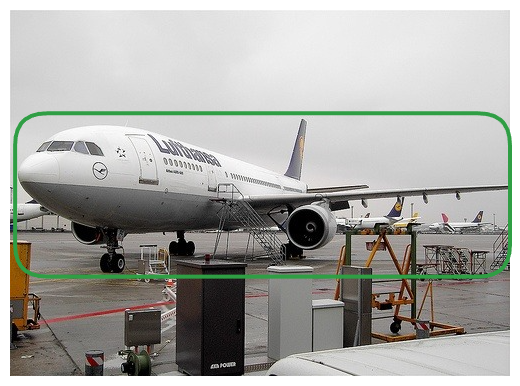
\includegraphics[width=\textwidth]{Figures/voc}\\
            \tiny(a) Pascal VOC (\cite{everingham2010pascal})
        \end{subfigure}
        \hspace{1cm}
        \begin{subfigure}{0.3\textwidth}
            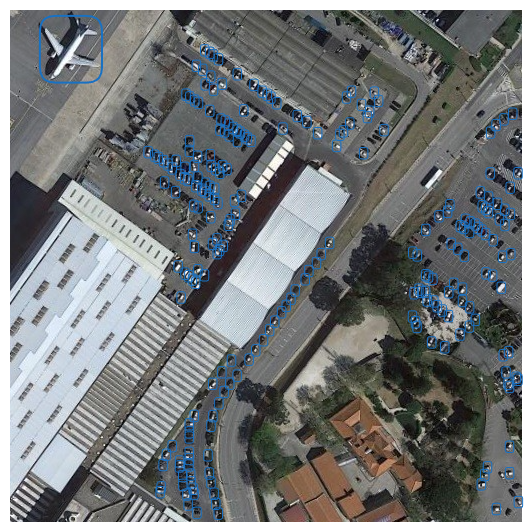
\includegraphics[width=0.75\textwidth]{Figures/dota}\\
            \tiny(b) DOTA (\cite{xia2018dota})
        \end{subfigure}
        \vspace{-1mm}
        \caption{Deux images issues des datasets DOTA (\cite{xia2018dota}) et Pascal VOC (\cite{everingham2010pascal}) illustrent la différence de taille entre des images aériennes et naturelles.}
    \end{figure}
    \vspace{-5mm}

    \begin{figure}
        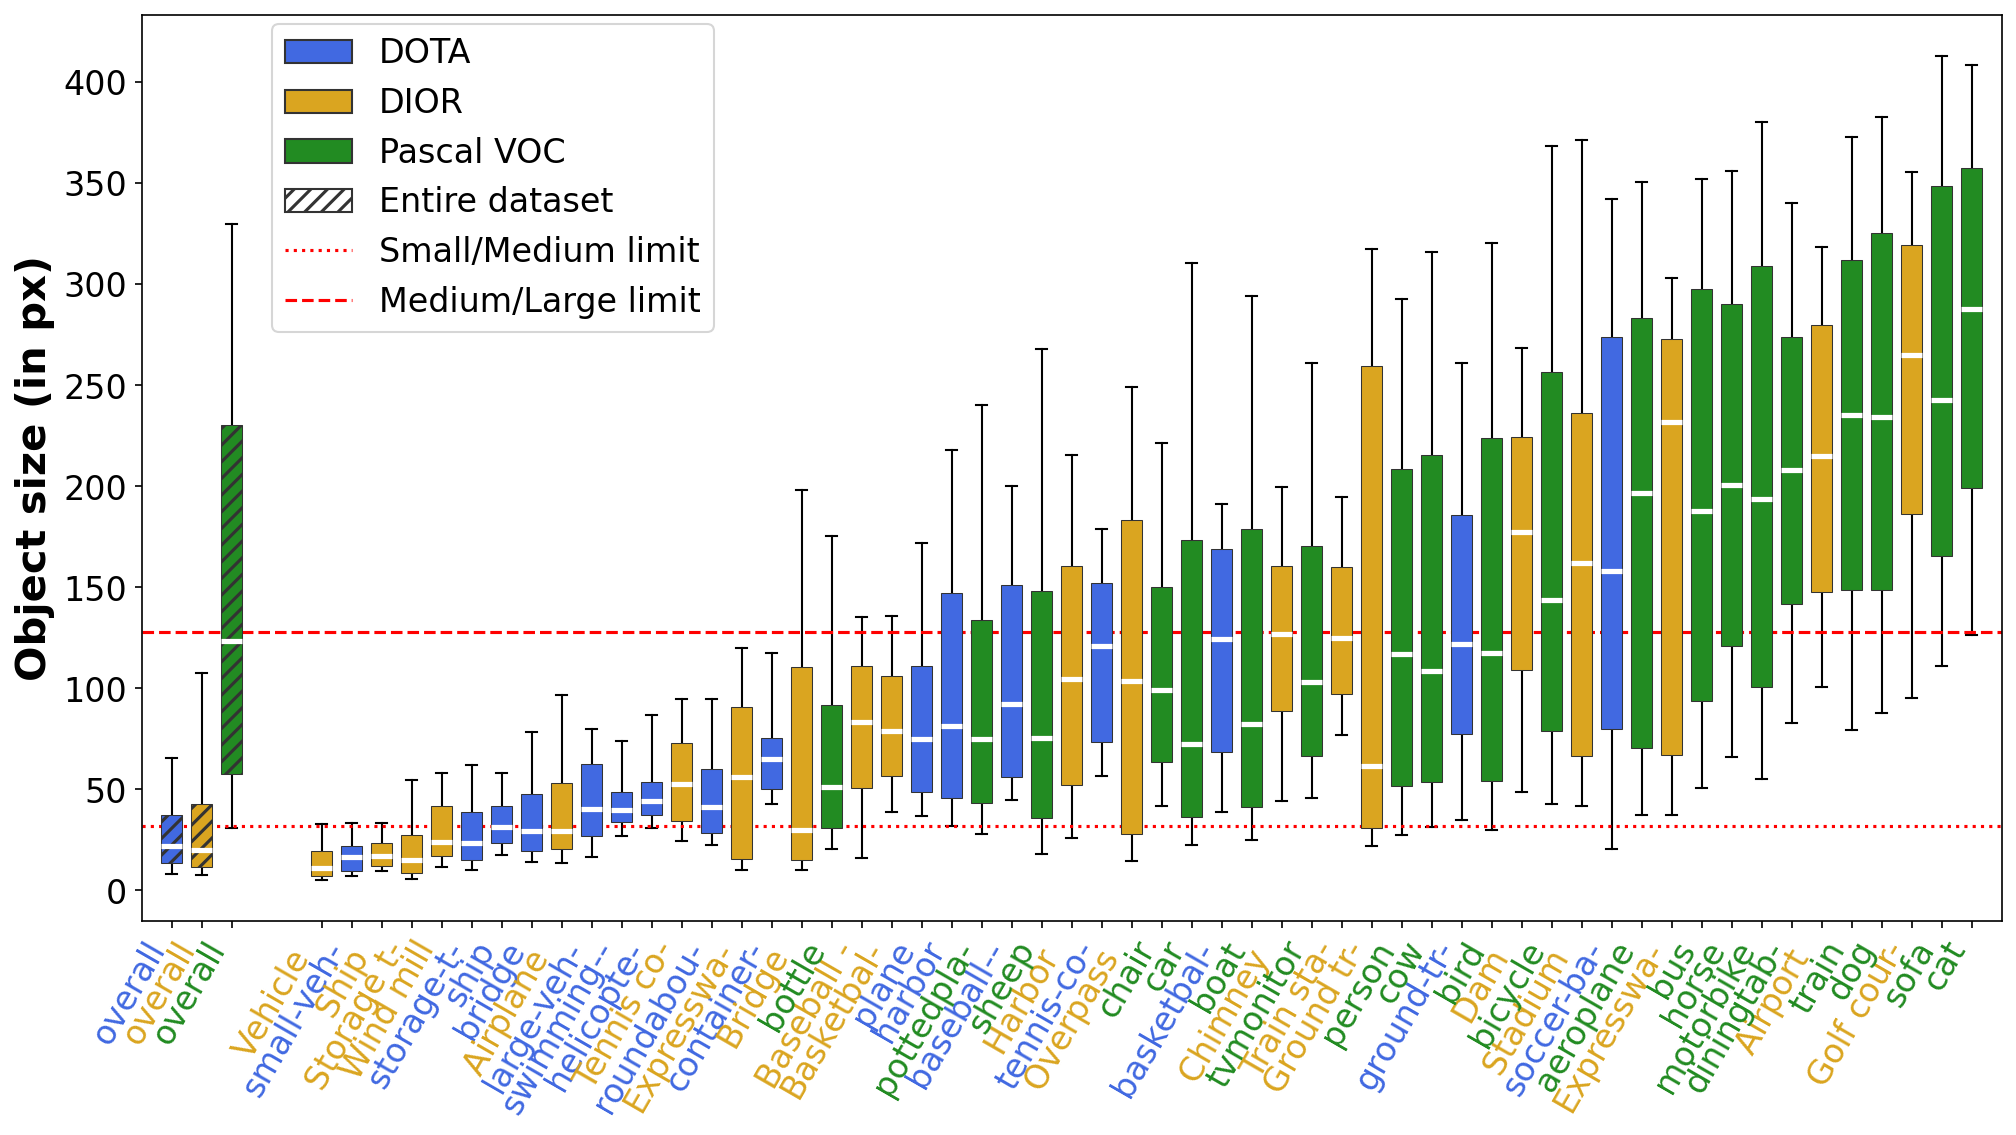
\includegraphics[width=0.6\textwidth]{Figures/object_sizes.png}
        \caption{Diagramme en boîte des tailles d'objets dans DOTA (\cite{xia2018dota}), DIOR (\cite{li2020object}) et Pascal VOC (\cite{everingham2010pascal}); par classe \textbf{(à droite)} et globalement \textbf{(à gauche)}.}
    \end{figure}


\end{subsectionframemod}